%-------------------------------------------------------------------------------
% File: testplan.tex
%
% Author: Marco Pinna
%         Created on <date>
%-------------------------------------------------------------------------------
\chapter{Test-plan and testbench}\label{ch:testplan}
The design of each component was followed by a testing phase performed via testbench modules, also written in VHDL, to ensure that said component was designed properly. Only the testbench of the final CRC modules will be presented in this chapter. Please refer to the repository for the rest of them.\\
\hfill \break
All the simulations of the testbenches were performed on \textit{ModelSim - Intel FPGA Starter Edition v. 2020.1}.\\

\section{CRC testbench}
As mentioned in \ref{sec:CRC_LUT.vhd}, the set of input and output ports of the CRC is the same, regardless of the implementation, because of the compliance with the specifications. This naturally led to a single testbench that could test both versions.\\
\hfill \break
A Python script was used to generate 10 random 7 bytes long messages and compute the CRC of each of them.
\begin{itemize}
	\setlength{\itemsep}{1pt}
  	\setlength{\parskip}{0pt}
  	\setlength{\parsep}{0pt}
	\item[-] \texttt{0526abfa59289d 75}
	\item[-] \texttt{1ad743298a5b0c 13}
	\item[-] \texttt{49dbf2d3fca778 7a}
	\item[-] \texttt{58de7943c3b4e1 f7}
	\item[-] \texttt{7a32768bdb8fb4 58}
	\item[-] \texttt{8d73243271fdf2 86}
	\item[-] \texttt{c387f7b71ddd50 2e}
	\item[-] \texttt{d8c66625791098 b7}
	\item[-] \texttt{e34a300fa4c345 1d}
	\item[-] \texttt{f9e70f4d2b6ed3 89}
\end{itemize}
\pagebreak
The testbench consists of three phases:
\begin{itemize}
	\item sender mode
	\item receiver mode with intact messages and correct CRCs
	\item receiver mode with corrupted messages
\end{itemize}
During the first phase \texttt{MD} is equal to \texttt{0} and the 10 random messages are input in succession. The output should show each of the 10 messages, in succession, and the correct CRC as the least significant byte.\\
During the second phase, \texttt{MD} is equal to \texttt{1} and the input consists of the 10 random messages each with its own CRC attached, in succession. The output should show each of the 10 messages, in succession, and the least significant byte equal to \texttt{0x00}.
The third phase is equal to the second phase, except for the output which should show non-zero values, proving the error detecting properties of the CRC algorithm.\\
Below are some screenshots from the testing phase on Modelsim.\\

\begin{figure}[H]
    \begin{center}
        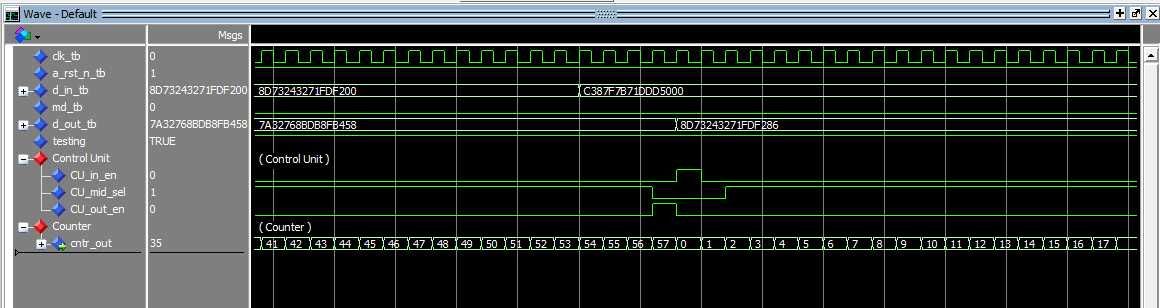
\includegraphics[scale=.6,clip]{img/test_bit_phase1.png}
    \end{center}
    \vspace*{-0.5cm}
    \caption{Testbench simulation of the bitwise architecture (phase 1)}
    \label{fig:test_bit_phase1}
\end{figure}

\begin{figure}[H]
    \begin{center}
        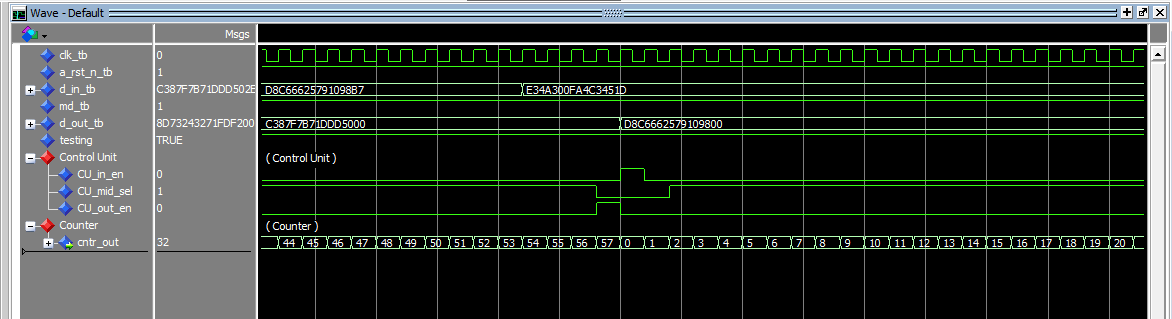
\includegraphics[scale=.6,clip]{img/test_bit_phase2.png}
    \end{center}
    \vspace*{-0.5cm}
    \caption{Testbench simulation of the bitwise architecture (phase 2)}
    \label{fig:test_bit_phase2}
\end{figure}

\begin{figure}[H]
    \begin{center}
        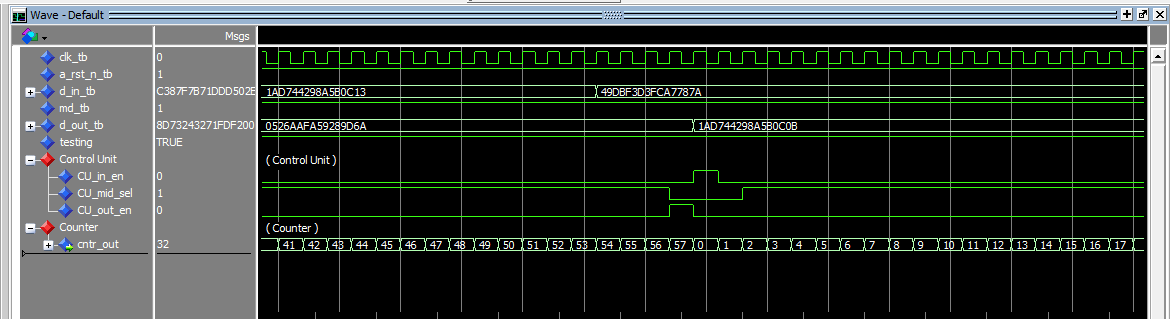
\includegraphics[scale=.6,clip]{img/test_bit_phase3.png}
    \end{center}
    \vspace*{-0.5cm}
    \caption{Testbench simulation of the bitwise architecture (phase 3)}
    \label{fig:test_bit_phase3}
\end{figure}

\begin{figure}[H]
    \begin{center}
        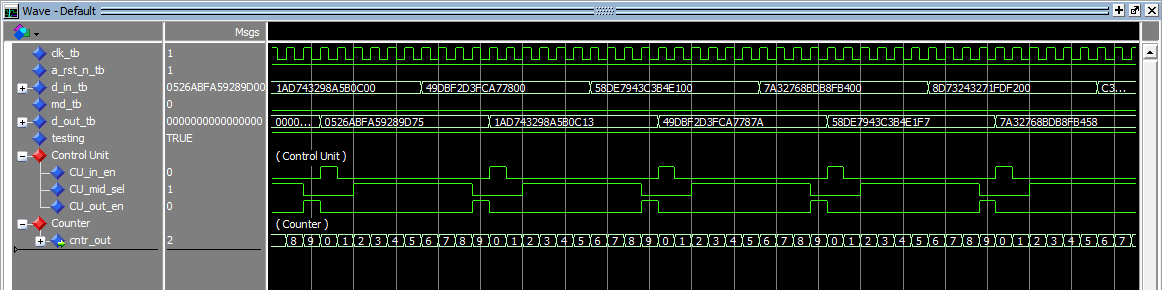
\includegraphics[scale=.6,clip]{img/test_lut_phase1.png}
    \end{center}
    \vspace*{-0.5cm}
    \caption{Testbench simulation of the LUT-based architecture (phase 1)}
    \label{fig:test_lut_phase1}
\end{figure}

\begin{figure}[H]
    \begin{center}
        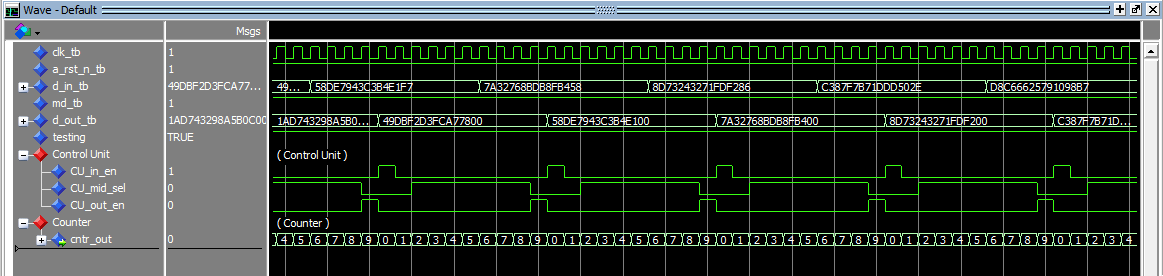
\includegraphics[scale=.6,clip]{img/test_lut_phase2.png}
    \end{center}
    \vspace*{-0.5cm}
    \caption{Testbench simulation of the LUT-based architecture (phase 2)}
    \label{fig:test_lut_phase2}
\end{figure}

\begin{figure}[H]
    \begin{center}
        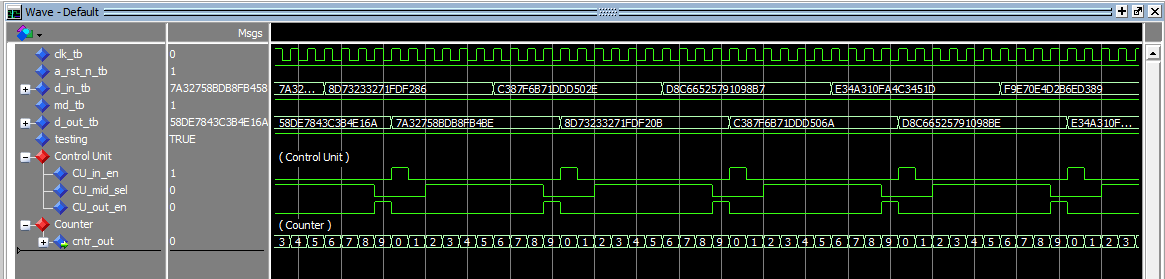
\includegraphics[scale=.6,clip]{img/test_lut_phase3.png}
    \end{center}
    \vspace*{-0.5cm}
    \caption{Testbench simulation of the LUT-based architecture (phase 3)}
    \label{fig:test_lut_phase3}
\end{figure}